\documentclass[a4paper]{jpconf}
\bibliographystyle{iopart-num}
\usepackage{graphicx}
\usepackage{hyperref}
\usepackage{cleveref}
\begin{document}

    \crefname{equation}{Equation}{Equations}%
    \crefname{chapter}{Chapter}{Chapters}%
    \crefname{section}{Section}{Sections}%
    \crefname{appendix}{Appendix}{Appendices}%
    \crefname{enumi}{Item}{Items}%
    \crefname{footnote}{Footnote}{Footnotes}%
    \crefname{figure}{Figure}{Figures}%
    \crefname{table}{Table}{Tables}%
    \crefname{theorem}{Theorem}{Theorems}%
    \crefname{lemma}{Lemma}{Lemmas}%
    \crefname{corollary}{Corollary}{Corollaries}%
    \crefname{proposition}{Proposition}{Propositions}%
    \crefname{definition}{Definition}{Definitions}%
    \crefname{result}{Result}{Results}%
    \crefname{example}{Example}{Examples}%
    \crefname{remark}{Remark}{Remarks}%
    \crefname{note}{Note}{Notes}%

\title{Numerical simulation of turbulent flow in a cyclonic separator}

\author{Dmitry Bogdanov and Sergey Poniaev}

\address{Division of Plasma Physics, Atomic Physics and Astrophysics, Ioffe Physical Technical Institute, 26 Polytekhnicheskaya, St Petersburg 194021, Russian Federation}

\ead{\href{mailto:dimyriy.bogdanov@gmail.com}{dimyriy.bogdanov@gmail.com}}

\begin{abstract}
In this study a numerical simulation of turbulent flow of an air with dispersed particles is presented for cyclonic separator. Since the separator construction make it impossible to simulate the flow using the classic turbulent models due to high streamlines curvature, the curvature correction term was included in $k-\omega-SST$ turbulence model. Experimental data for turbulent flow in U-duct has been used for model validation. The numerical simulation results demonstrate that the implemented turbulence model successfully predicts the cyclonic separator efficiency.
\end{abstract}

\section{Introduction}
Cyclonic separators are widely used for gas separation from dispersed phase. Its efficiency calculated by dividing the number of filtered particles by the total number of particles. However, numerical simulation of the turbulent flow in separator for prediction of its efficiency is a very difficult problem since classic eddy-viscosity models can't adequately predict the flow\cite{ShurSpallart} due to high streamlines curvature and more specifically, inadequate calculation of turbulence kinetic energy production. The production can be corrected using Shur-Spalart curvature correction term for Spalart-Allmaras turbulence model reformulated\cite{Smirnov} in terms of the $k-\omega-SST$ turbulence model.

\section{Cyclonic separator model}
The typical scheme of air flow in cyclonic separator is presented on \cref{fig:physicalModel}.	
\begin{figure}[h]
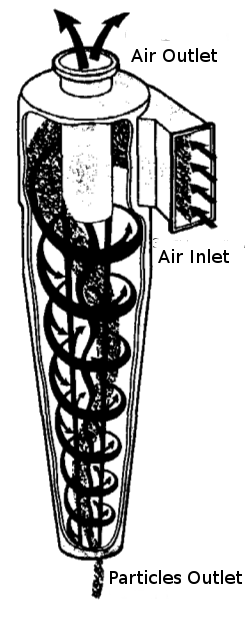
\includegraphics[width=14pc]{flowScheme1.png}\hspace{2pc}%
\begin{minipage}[b]{14pc}\caption{\label{fig:physicalModel}Scheme of the air flow inside cyclonic separator.}
\end{minipage}
\end{figure}

\section*{References}
\bibliography{iopart-num}
\end{document}


